\begin{enumerate}[label=\thesection.\arabic*.,ref=\thesection.\theenumi]
\numberwithin{equation}{enumi}
\item Which of the following is \textbf{incorrect} ?\\
(A) Lead compensator is used to reduce the settling time\\
(B) Lag compensator is used to reduce the steady state error\\
(C) Lead compensator may increase the order of a system\\
(D) Lag compensator always stabilzes an unstable system\\
\\
\solution Lead and Lag compensators - 
\\* \textbf{Lead compensator } - The lead compensator is an electrical network which produces a output having \textbf{phase lead} when a input is applied. 
\\
\begin{equation}
H(s) = \frac{s+z}{s+p}   0 \textless z \textless p
\centering
\end{equation}
\\* \textbf{\\Lag compensator} - The Lag Compensator is an electrical network which produces a  output having the \textbf{phase lag} when a input is applied.
\begin{equation}
H(s) = \frac{s+z}{s+p}  \hspace{1cm} 0 \textless p \textless z
\centering
\end{equation}


Lead compensators - 
The lead compensator circuit in the ‘s’ domain is shown in the following figure.
 
\begin{figure}[h]
 
\begin{subfigure}{0.5\textwidth}
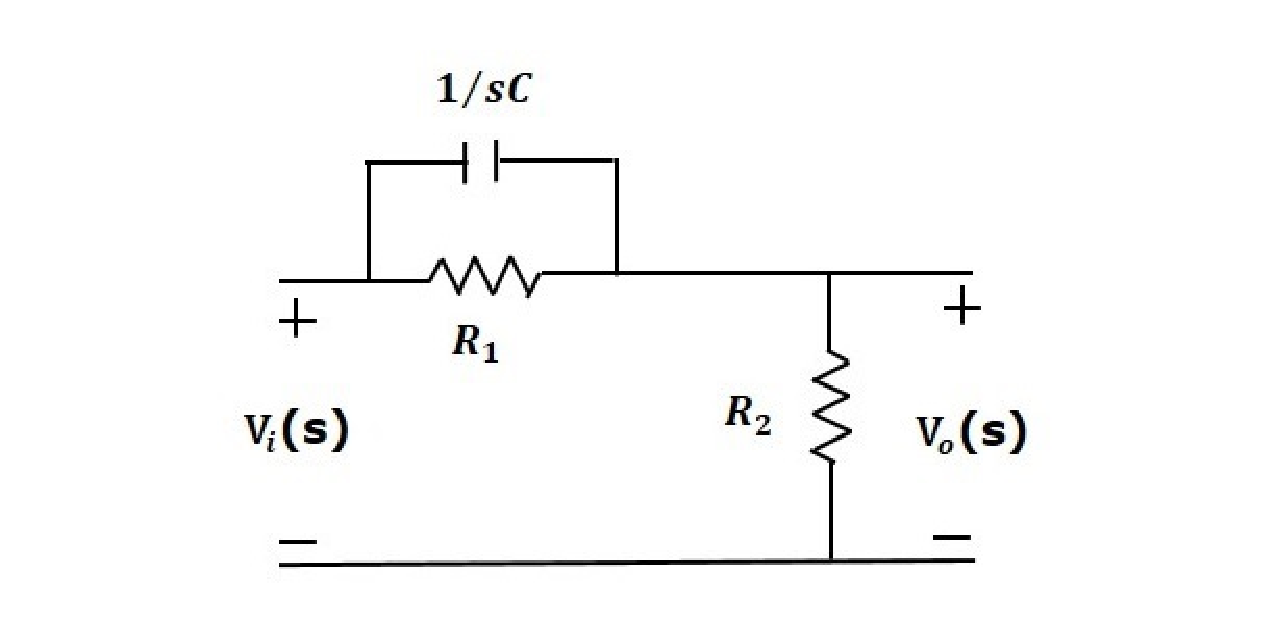
\includegraphics[width=0.9\linewidth, height=5cm ,inner]{./figs/ee18btech11027/lead_compensator.eps} 
\label{fig:subim1}
\end{subfigure}
\end{figure}


Lead compensator - 
The transfer function of this lead compensator is -
\begin{align}
    \frac{V_o(s)}{V_i(s)} = \beta  \frac{s \tau +1}{s\beta \tau +1} \\
where\\
\tau = R_1C  \beta =\frac{R_2}{R_1+R_2}
\end{align}

\vspace{0.3cm}substituting s=j\omega \\
\centering
\begin{equation}
\centering
 \frac{V_o(j\omega)}{V_i(j\omega)} = \beta  \frac{j\omega \tau +1}{j \omega\beta \tau +1}
\end{equation}
\\
\begin{align}
phase angle \phi = \tan^{-1} {(\omega\tau)} - \tan{-1}{(\omega\beta\tau)}\\
since 0 \textless \ \beta < 1\\
\phi > 0
\end{align}




Lag compensators - 
The lag compensator circuit in the ‘s’ domain is shown in the following figure.
 
\begin{figure}[h]
 
\begin{subfigure}{0.5\textwidth}
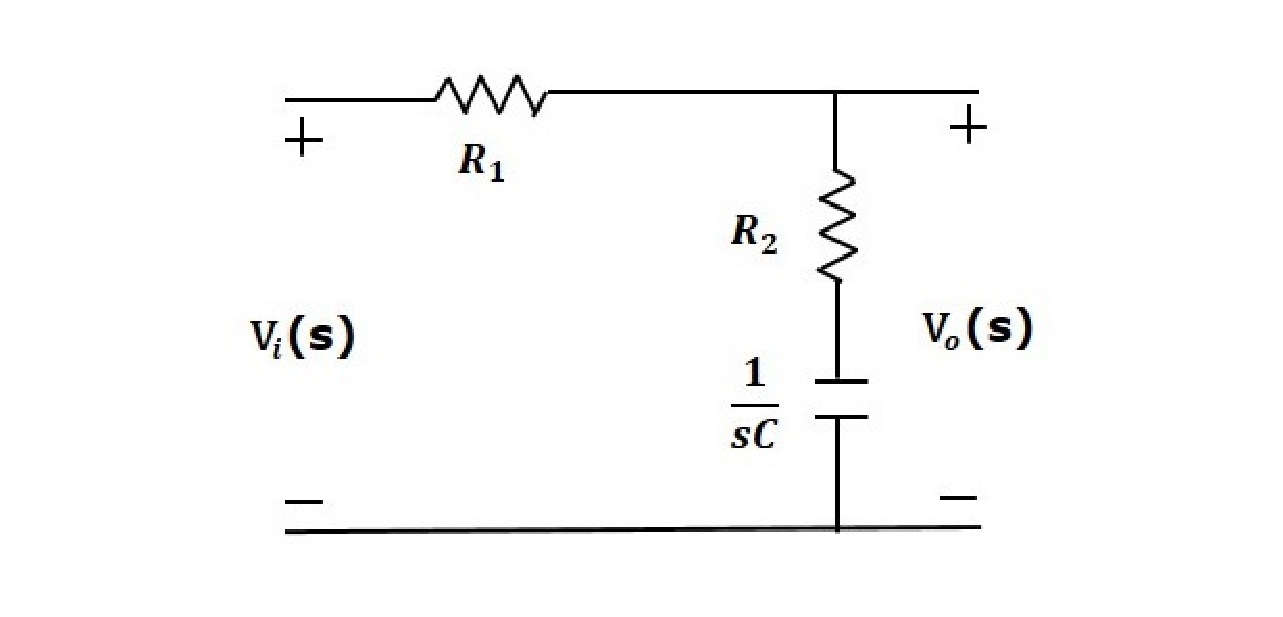
\includegraphics[width=0.9\linewidth, height=5cm ,inner]{./figs/ee18btech11027/lag_compensator.eps} 
\label{fig:subim1}
\end{subfigure}
\end{figure}

The transfer function of this lag compensator is -
\begin{align}
    \frac{V_o(s)}{V_i(s)} = \frac{1}{\alpha}  \frac{s + \frac{1}{\tau}}{s + \frac{1}{\alpha\tau}} \\
where\\
 \tau = R_2C  \alpha =\frac{R_1+R_2}{R_2}
\end{align}

substituting s=j\omega \\
\begin{equation}
\centering
 \frac{V_o(j\omega)}{V_i(j\omega)} = \frac{1}{\alpha}  \frac{j\omega + \frac{1}{\tau}}{j\omega + \frac{1}{\alpha\tau}}
\end{equation}
\begin{align}
phase angle \hspace{1cm}\phi = \tan^{-1} {(\omega\tau)} - \tan^{-1}{(\omega\alpha\tau)}\\
since \alpha > 1\\
\phi < 0
\end{align}


BODE PLOTS -
\begin{figure}[h]
 
\begin{subfigure}{\textwidth}
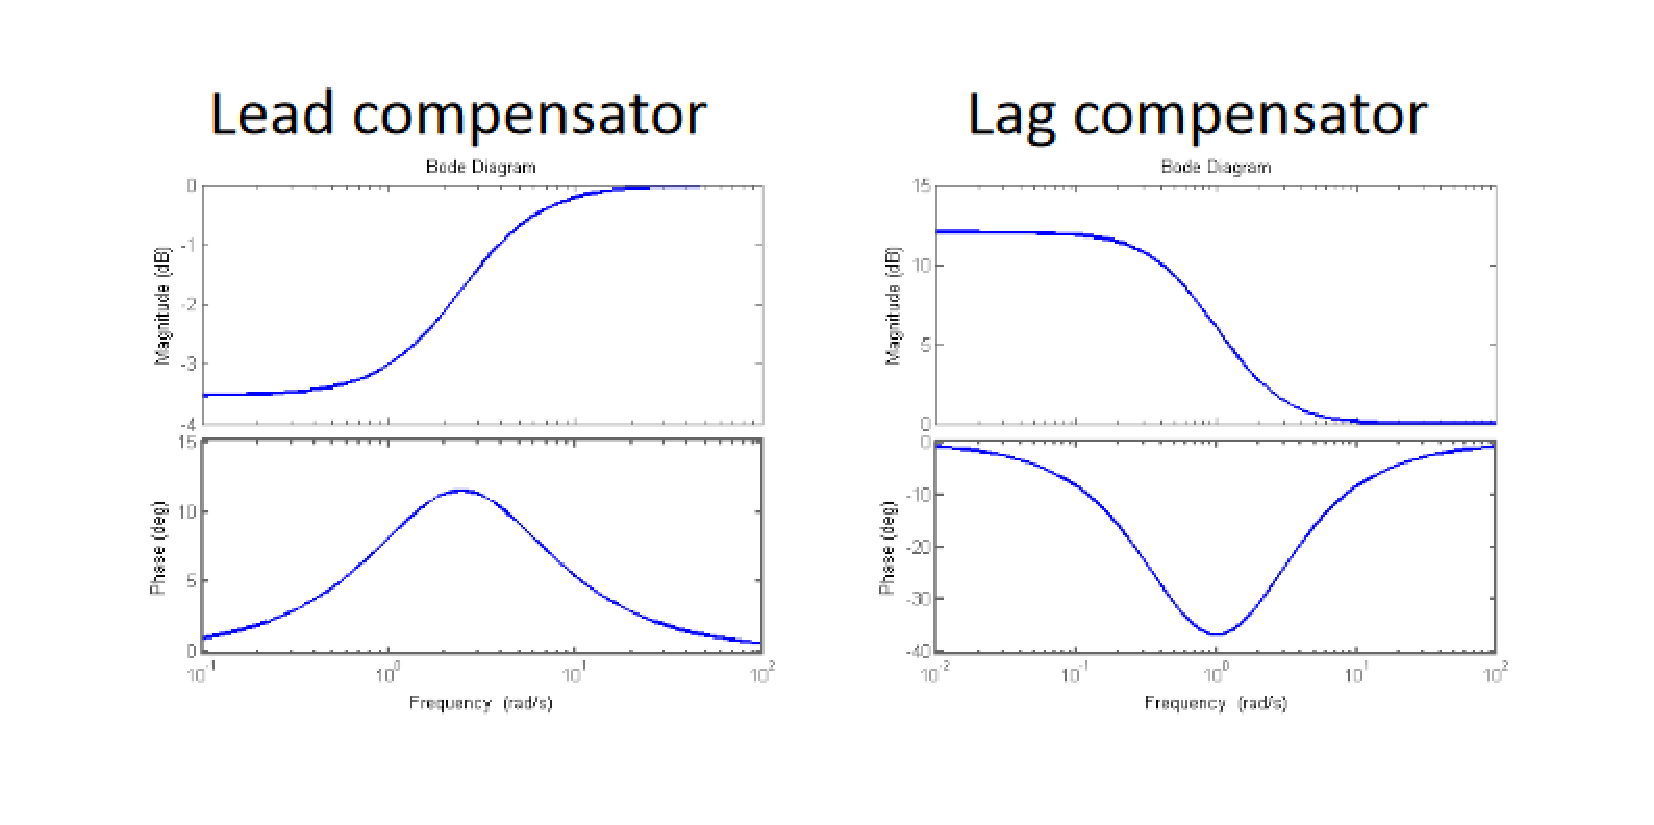
\includegraphics[width=1\linewidth, height=7cm ,inner]{./figs/ee18btech11027/Screen.eps} 
\label{fig:subim1}
\end{subfigure}
\end{figure}


Statement - A\\Lead compensator is used to reduce settling time.
Since lead compensator adds + phase for any value of frequency, the bode plot for phase vs frequency is above the one which is without lead compensator.\\

phase margin \phi_m = 180 + \phi_{gain = 0}\\
as\ lead\ compensator\ adds additional\ phase\ at\ all\ frequencies, \\
$\phi_{gain = 0}$ \ gets increased, and hence\ phase\ margin



Bode plot - increased phase margin - 
\begin{figure}[h]
 
\begin{subfigure}{\textwidth}
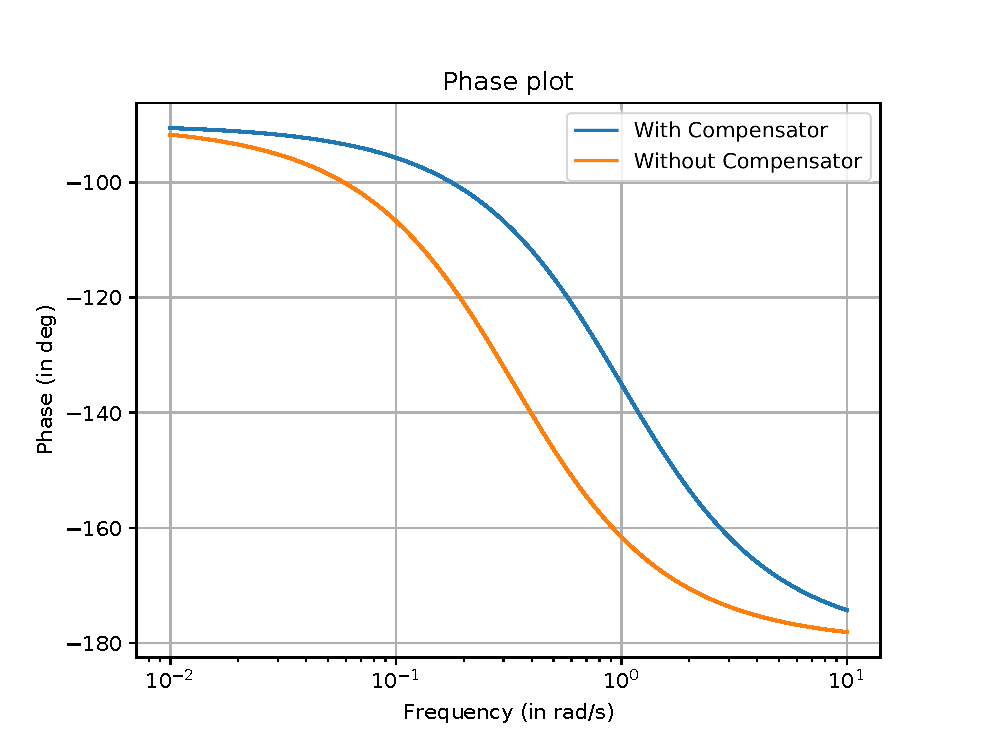
\includegraphics[width=1\linewidth, height=7cm ,inner]{./figs/ee18btech11027/lead_compensator_phase.eps} 
\label{fig:subim1}
\end{subfigure}
\end{figure}


Relation between phase margin and damping ratio
Now,
\zeta = 0.01 $\times$ \phi_m\\

from this we get that damping factor also increases.\\

\implies damping\ is\ increased \\

\implies settling\ time\ decreased\\



Relation between phase margin and damping ratio
Consider a second order system,\\

G(s) = {\huge{$\frac{\omega_n^2}{s^2+2\zeta\omega_ns+\omega_n^2} $}}\\
 using value of $\phi_m$ to solve for $\zeta$.\\

set 20 $\log{|G(s)|}$ = -3dB to solve for \omega_n\\

using this equations we get,\\

\phi_m = \tan^{-1}{\frac{2\zeta}{\sqrt{\sqrt{1+4\zeta^4} - 2\zeta^2}}}\\ \\
a handy relation is - \zeta = 0.01\phi_m\\

\begin{figure}[h]
 
\begin{subfigure}{\textwidth}
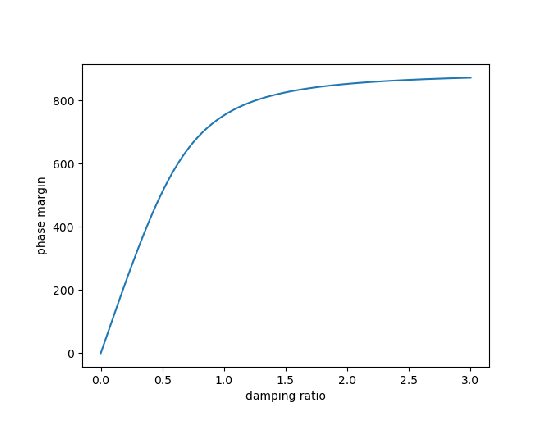
\includegraphics[width=1\linewidth, height=7cm ,inner]{./figs/ee18btech11027/realtion.eps} 
\label{fig:subim1}
\end{subfigure}
\end{figure}

    



Time response - reduced settling time - 
\begin{figure}[h]
 
\begin{subfigure}{\textwidth}
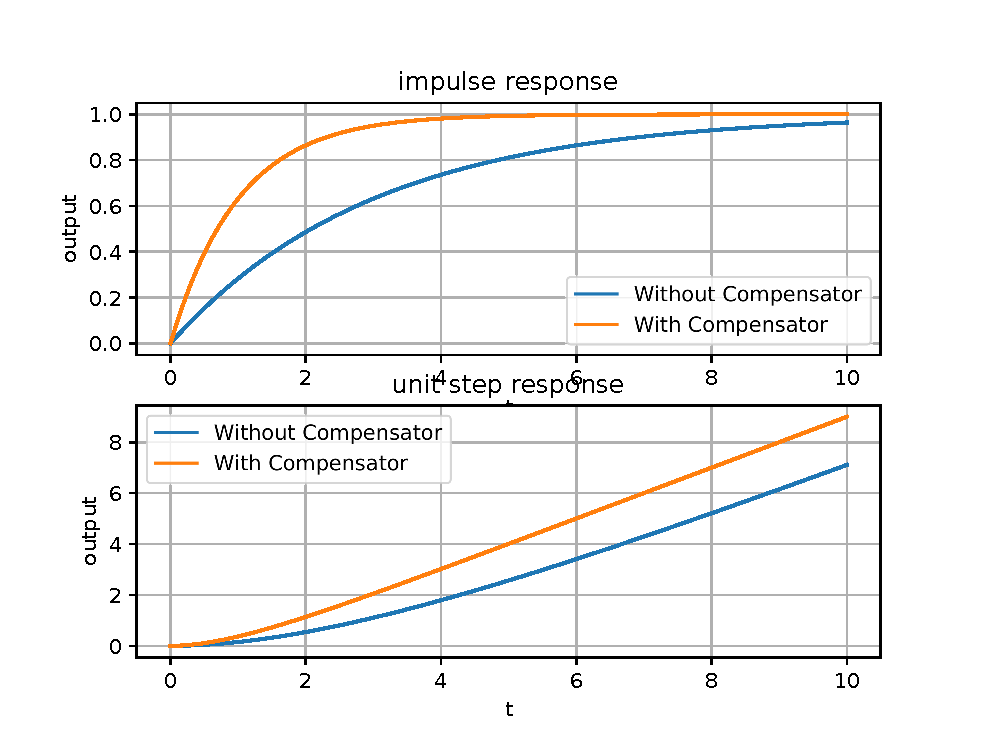
\includegraphics[width=1\linewidth, height=7cm ,inner]{./figs/ee18btech11027/settling_time.eps} 
\label{fig:subim1}
\end{subfigure}
\end{figure}

    
Statement - B\\Lag compensator is used to reduce the steady state error
From the bode plot it is clear that the lag compensator has an high gain for low frequencies.
since steady state error is given by - 
\begin{equation}
    e(\infty) = \lim_{s\to0} \frac{sR(s)}{1+G(s)}
\end{equation}
\begin{figure}[h]
 
\begin{subfigure}{\textwidth}
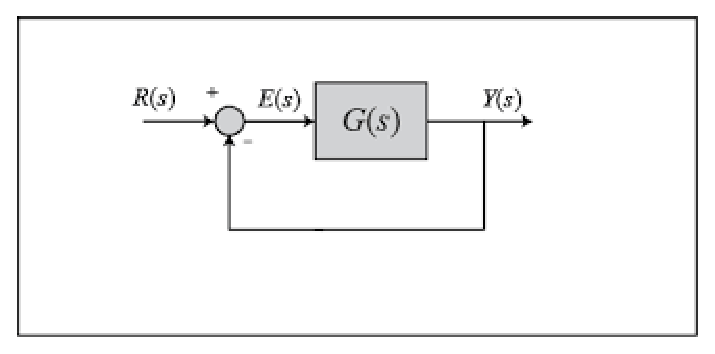
\includegraphics[width=1\linewidth, height=4cm ,inner]{./figs/ee18btech11027/unity.eps} 
\label{fig:subim1}
\end{subfigure}
\end{figure}



for low frequencies - the gain is high \implies G(s) \to \large number\\
\implies e(\infty) \to smaller value\\
\implies steady\ state\ error\ decreases \\
\begin{figure}[h]
 
\begin{subfigure}{\textwidth}
\includegraphics[width=1\linewidth, height=4cm ,inner]{./figs/ee18btech11027/table.eps} 
\label{fig:subim1}
\end{subfigure}
\end{figure}


Verification - 
Let the system transfer function be -
\begin{equation}
   c(s)= \frac{1}{s+2}
\end{equation}
and the lag compensator be- 
\begin{equation}
   t(s)= \frac{s+3}{s+1}
\end{equation}
therefore resulting system transfer function-
\begin{equation}
    G(s) = \frac{s+3}{(s+2)(s+1)}
\end{equation}

Hence steady state error for unit step input,\\

Without lag compensator = $\frac{1}{1+c(s)}$ \\

as s \to 0
\implies $E_{ss} = \frac{1}{1+0.5}$  \implies E_{ss} = 0.66\\

With lag compensator = $\frac{1}{1+G(s)}$\\

as s \to 0
{\implies} $E_{ss} = \frac{1}{1+1.5}$  \implies E_{ss} = 0.4
\\

Statement - C\\Lead compensator may increase the order of a system
since the transfer function adds a pole and a zero therefore it may increase the order of a system.\\
For example -

\centering
G(s) = $\frac{1}{s+2}$\\
D(s) = $\frac{s+1}{s+3}$\\

G(s)\textbf{.}D(s) = $\frac{s+1}{(s+2)(s+3)}$\\

G(s)\textbf{.}D(s) = $\frac{s+1}{s^2+5s+6}$\\

\begin{flushleft}
Maximum power in denominator = 2\\
Hence order increased to 2 from 1
\end{flushleft}

\\
Statement - D\\ Lag compensator always stabilizes an unstable system
\begin{flushleft}
This statement is wrong.\\
If a system has a pole on right side of s plane, lag compensator cannot stabilize those systems. This is because the resulting system also has an pole on the right side of s plane.
\end{flushleft}
\begin{align}
$R(s) = \frac{1}{s-2}$\\

$G(s) = \frac{s+3}{s+1}$\\
$R(s)\textbf{.}G(s) = \frac{(s+3)}{(s-2)(s+1)}$\\ \\
output = 1.66e^{(2t)} + 0.66e^{(-t)}
\end{align}

\textbf{}\begin{figure}[h]
 
\begin{subfigure}{\textwidth}
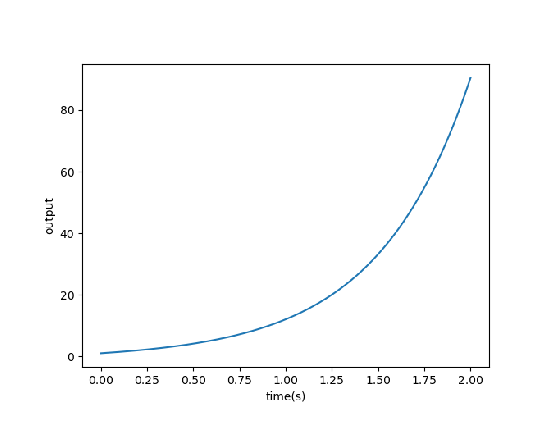
\includegraphics[width=1.05\linewidth, height=8cm ,inner]{./figs/ee18btech11027/unstable.eps} 
\label{fig:subim1}
\end{subfigure}
\end{figure}


\end{enumerate}